\documentclass[]{spie}  %>>> use for US letter paper
%\documentclass[a4paper]{spie}  %>>> use this instead for A4 paper
%\documentclass[nocompress]{spie}  %>>> to avoid compression of citations

\renewcommand{\baselinestretch}{1.0} % Change to 1.65 for double spacing
\newcommand*\mean[1]{\bar{#1}}
 
\usepackage{amsmath,amsfonts,amssymb}
\usepackage{graphicx}
\usepackage[colorlinks=true, allcolors=blue]{hyperref}
\usepackage{textcomp}
\usepackage{gensymb}
\usepackage{color,soul}

%\usepackage[justification=left]{caption}
\usepackage{multirow}
\usepackage{booktabs}
\usepackage{natbib}
\usepackage{subfig}
%\usepackage[caption=false]{subfig}
%\usepackage[left]{lineno}
%\linenumbers

\renewcommand{\arraystretch}{1.3}

\title{Point Spread Function Reconstruction on the OSIRIS Imager}

\author[a,*]{Sean K. Terry}
\author[a]{Jessica R. Lu}
\author[b]{Anna Ciurlo}

\affil[a]{Department of Astronomy, University of California, Berkeley, CA 94720, USA}
\affil[b]{Division of Astronomy \& Astrophysics, University of California Los Angeles, CA 90095, USA}

% Option to view page numbers
\pagestyle{plain} % change to \pagestyle{plain} for page numbers   
%\setcounter{page}{301} % Set start page numbering at e.g. 301
 
\begin{document}
\pagecolor{white}
\maketitle

\begin{abstract}
The Keck All-sky Precision Adaptive Optics (KAPA) project will deliver significant upgrades to the Keck-I adaptive optics (AO) system. In addition to hardware upgrades, a suite of PSF-reconstruction software is also being developed for the next-generation AO system. In this study we aim to model PSF variations for the OSIRIS imager using knowledge from instrumental aberration calibrations and atmospheric turbulence modeling. We use phase diversity measurements obtained with a calibration fiber source to characterize the instrumental aberrations across the OSIRIS field of view, and report its variation over time. We find the wavefront error varies by XX nm on a daily basis, however the differential aberrations across the field of view vary by less than YY nm, implying that off-axis instrumental aberrations need only be measured between openings (e.g. hardware upgrades) of the OSIRIS instrument. Finally, we develop a novel version of the AIROPA PSF-R software package to analyze simulated images and on-sky galactic center (GC) images taken with the OSIRIS imager. We compare astrometric and photometric precision between the single-PSF and variable-PSF modes in AIROPA, finding that on average the precision is YYY.
\end{abstract}

% Include a list of keywords after the abstract 
\keywords{adaptive optics -- PSF reconstruction, photometry, astrometry}

{\noindent\footnotesize\textbf{*} \href{mailto:sean.terry@berkeley.edu}{sean.terry@berkeley.edu}}

\section{Introduction} \label{sec:intro}
Large ground-based observatories the utilize adaptive optics (AO) have been delivering diffraction-limited imaging at infrared wavelengths for several decades now. While high-resolution imaging using AO has enabled revolutionary science results (stars orbiting Sgr A$^*$, directly imaged exoplanets, strong gravitational lensing, etc), some limitations have persisted. These are largely related to the anisoplanatic effect as observed on single-conjugate AO systems. With a single laser guide star (LGS), the AO correction degrades, sometimes rapidly, as the distance from the LGS increases. This ultimately causes the point spread function (PSF) to vary with both time and position in the field of view, which can be difficult to accurately characterize.\\
\indent The Anisoplanatic and Instrumental Reconstruction of Off-axis PSFs for AO (AIROPA) is a suite of software packages that utilizes phase-diversity measurements, atmospheric profile data, and wave propagation through both turbulence and optical systems. With this knowledge, AIROPA generates a model of the field-dependent PSF for both natural guide star (NGS) and laser guide star (LGS) modes. The software functions under the assumption that every PSF that is extracted consists of a convolution of the on-axis PSF, the instrumental aberration, and the atmospheric anisoplanatism \cite{do:2018a}.\\
\indent While there are several promising ongoing programs to upgrade the AO systems on both Keck telescopes \cite{wizinowich:2020a, bond:2020a}, modeling and understanding the time-dependent and spatial variability of the PSF remains an important task for next-generation AO systems. This study supports the development of PSF-R techniques to be used for the new Keck All-sky Precision Adaptive Optics (KAPA) system onboard Keck-I, which is scheduled to see first light in 2024. The primary KAPA upgrades include a new laser system with a high-powered TOPTICA 22W laser, new beam train infrastructure for generating an asterism of four LGS that will allow for laser tomography AO (LTAO), an infrared tip-tilt sensor (TRICK), a new real-time controller (RTC) computer and wavefront sensor camera that can run significantly faster than the previous system.\\
\indent The current AO system configuration at Keck-I has the AO bench and OSIRIS instrument situated on a Naysmith platform to the left of the telescope. The AO wavefront sensing is performed either on a single bright natural guide star or a LGS using a Shack-Hartmann wavefront sensor that operates at visible wavelengths ($\lambda_c {\sim}655$nm). In the LGS case, the correction is made on a single artificial star typically at the center of the field of view. This means that the system corrects for the total integrated atmospheric turbulence \cite{wizinowich:2006a} along a cone emanating from the LGS which is at a fixed distance of 90km above the telescope (e.g. sodium isotope stratospheric layer). The OSIRIS instrument itself is composed of an integral field spectrograph (IFS) and an imager with a 2046$\times$2046 H2RG detector. The detector plate scale is 10 mas/pixel, giving an effective total field of view of 20.4'' $\times$ 20.4''. Finally, the imager can operate concurrently or independently of the spectrograph, and each instrument has its own filter wheel(s).\\
\indent AIROPA was originally developed for the near-infrared camera 2 (NIRC2) on the Keck-II telescope \citep{witzel:2016a}. Further descriptions of the software are presented in a series of recent papers which describe modeling the NIRC2 instrumental aberrations as a function of time, testing AIROPA with calibration data, as well as simulation tests and applying AIROPA to several on-sky science datasets \citep{ciurlo:2022a, turri:2022, terry:2023a}. \\
\indent This paper is organized as follows: In Section \ref{sec:phase_diversity}, we characterize the instrumental aberrations on the OSIRIS detector across two epochs. In Section \ref{sec:simulations} we present our AIROPA analysis and results using several simulated images. Section \ref{sec:on_sky_obs} describes our analysis of real on-sky OSIRIS data for the galactic center (GC). In Section \ref{sec:results}, we analyze the effectiveness of AIROPA to reconstruct the spatially variable PSF for OSIRIS and compare the results to the static PSF mode. Finally, we give a discussion and conclude the paper in Section \ref{sec:conclusion}.

\section{Phase Diversity}\label{sec:phase_diversity}
Phase diversity measurements are taken during afternoon calibrations on both NIRC2 and OSIRIS AO benches. First, a fiber source that is mounted on a stage at the entrance to the AO system is centered at the OSIRIS pointing origin (i.e. approximately at the center of the detector). The fiber is imaged while it is in-focus and additionally at three subsequent out-of-focus levels ($+$5mm, $-$5mm, and $-$10mm). The purpose of these daily measurements is to obtain information about the instrumental aberrations within the AO system, and to make corrections to the DM and other components in order to optimize the system stability for subsequent nightly observing. This process is sometimes referred to as `image sharpening'. For OSIRIS, we use the following setup: \texttt{instrument-imager}, \texttt{BrGamma} filter ($\lambda_c = 1.686 \mu$m), and \texttt{open-pupil}.\\
\indent There are some limitations from the fiber for these calibrations, namely that the fiber illumination is not perfectly uniform and slightly varies between exposures. We implement schemes that were previously developed for NIRC2 phase diversity as described in \cite{ciurlo:2022a} to mitigate some of these issues and produce well-behaved fiber images. Particularly, we use various neutral density filters in front of the fiber source to dim or enhance the light, since the luminosity of the fiber has measurable variation and its light is spread over a larger number of pixels for the more out-of-focus positions. Further, the integration times are modified for the different focus levels to optimize signal-to-noise and avoid saturation. The target signal-to-noise ratio we achieve for the fiber image at each focus level is 20. This process is repeated at each position across the detector to characterize the filed-dependent instrumental aberrations. Finally, we take background images with the fiber turned off and flat field images for calibration purposes. \\
\indent Figure XXXYYY shows an example of the in-focus and out-of-focus fiber images from the 2020 data. The top row shows the fiber images at the central detector position, while the bottom row shows the fiber images near the lower-left corner detector position. The phase diversity observations presented in this work were taken in 2020 and 2021 and are presented in Table 1. It is worth noting that OSIRIS was opened several times between the 2020 and 2021 observations (central phasemap significantly different between years).

\begin{table}[!h]
\centering
\caption{Phase diversity data obtained for instrumental aberrations on OSIRIS.}
\begin{center}
\begin{tabular}{lccccc}
\hline
        Date [UT] &  N Pos &  WFE$_{\textrm{Cen}}$ [nm] &  WFE$_{\textrm{Lower-left}}$ [nm] & WFE$_{\textrm{Cen}-\textrm{LL}}$ [nm] \\\hline\hline
        2020 Aug 21 & 25 & NNN & OOO & aaa\\
        2021 Oct 06 & 81 & MMM & PPP & bbb\\\hline
\end{tabular}
\end{center}
{\raggedright \footnotesize{\textbf{Note}. N Pos gives the total number of positions observed, the wavefront error at the center (\textit{Cen}), lower-left corner (\textit{Lower-left}), and the difference between the center and lower-left (\textit{Cen}$-$\textit{LL}).}\par}
\label{tab:fields-metrics}
\end{table}

\begin{figure}[!h]
 \hspace{1cm}
 \makebox[\textwidth][c]{
 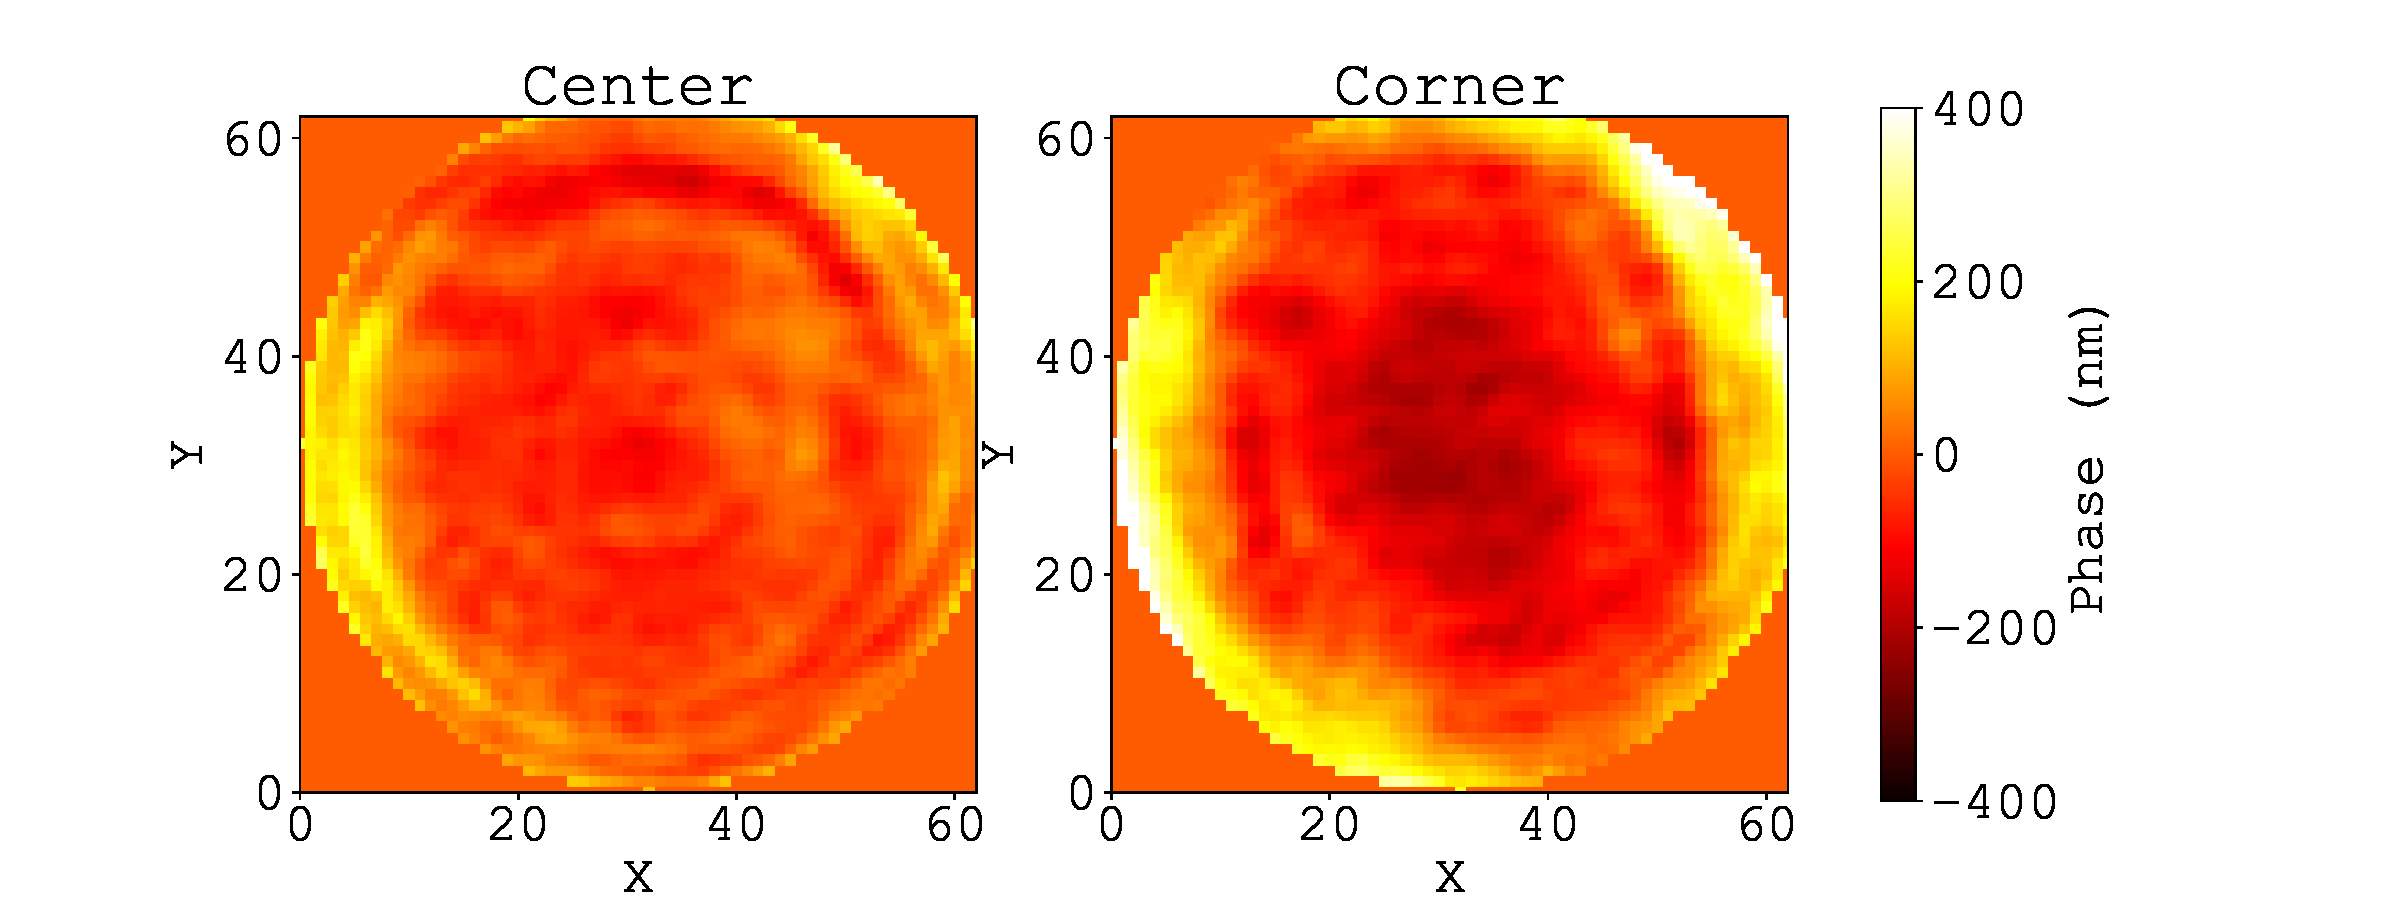
\includegraphics[width=1.1\textwidth]{airopa/Figures/osiris_cencorn_grid.pdf}
 }
 \caption{\footnotesize Center and corner phase maps for the OSIRIS detector taken in 2020. Both phase maps are on the same color scale (in nm). \label{fig:phase-map-cencorn}}
\end{figure}

\begin{figure}[!h]
 \hspace{5mm}
 \makebox[\textwidth][c]{
 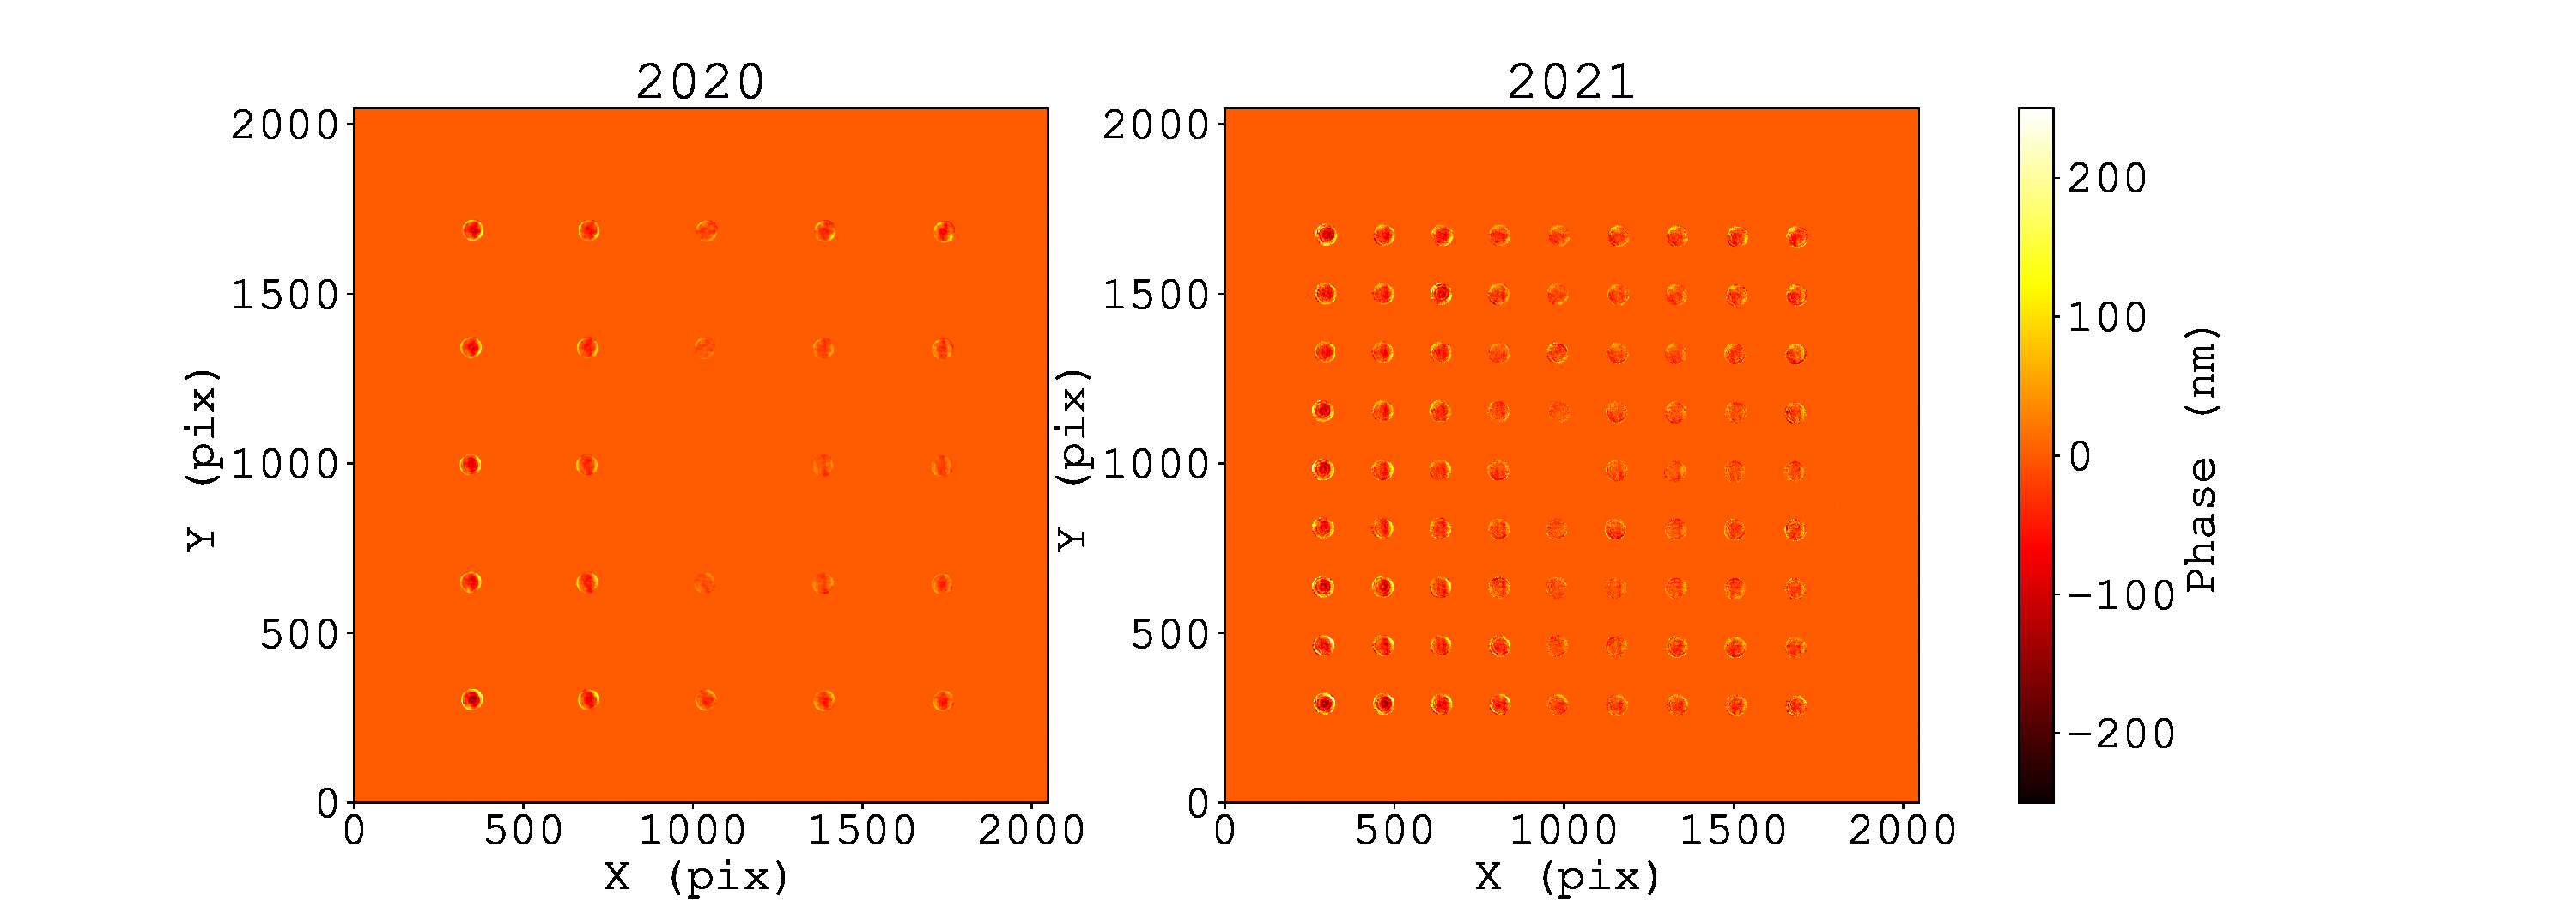
\includegraphics[width=1.4\textwidth]{airopa/Figures/osiris_phasemap_grid_compare.pdf}
 }
 \caption{\footnotesize Center-subtracted phase map grid for the OSIRIS detector from data obtained in 2020 (\textit{left}) and 2021 (\textit{right}). \label{fig:phase-map-grid}}
\end{figure}

\subsection{Phase Map Retrieval} \label{subsec:phase_map_retrieval}
\indent The daily image sharpening procedure is only performed at the central position on the detector. In order to characterize the phase aberrations as a function of detector position, we iteratively move the fiber to positions along a grid on the detector and take subsequent in-focus and out-of-focus images (see left panel of Figure \ref{fig:grid_stars} for a reference). retrieve the wavefront phase from the intensity maps of the in and out-of-focus fiber sources using the Gerchberg-Saxton algorithm \cite{gerchberg:1972a}. Figure ZZZ shows the central and lower-left corner phase maps for the OSIRIS detector with data from 2020-08-21. The central phase map is smoother compared to the corner map, and has a smaller RMS variation of ${\sim}100$nm compared to the corner phase map with an RMS variation of  Figure \ref{fig:phase-map-grid} shows a $5\times5$ grid of phase maps from 2020 as well as a $9\times9$ grid from 2021, with the central phase map subtracted from each.

\section{Simulations} \label{sec:simulations}
We use AIROPA single-PSF and variable-PSF mode to analyze a grid of pinholes from the newly installed pinhole calibration unit (PCU). Figure ZZ shows the uniform grid of pinholes, the next figure will show the residual image created with the single-PSF mode alongside the residual image created with the variable-PSF.

\begin{figure}[!h]
 \makebox[\textwidth][c]{
 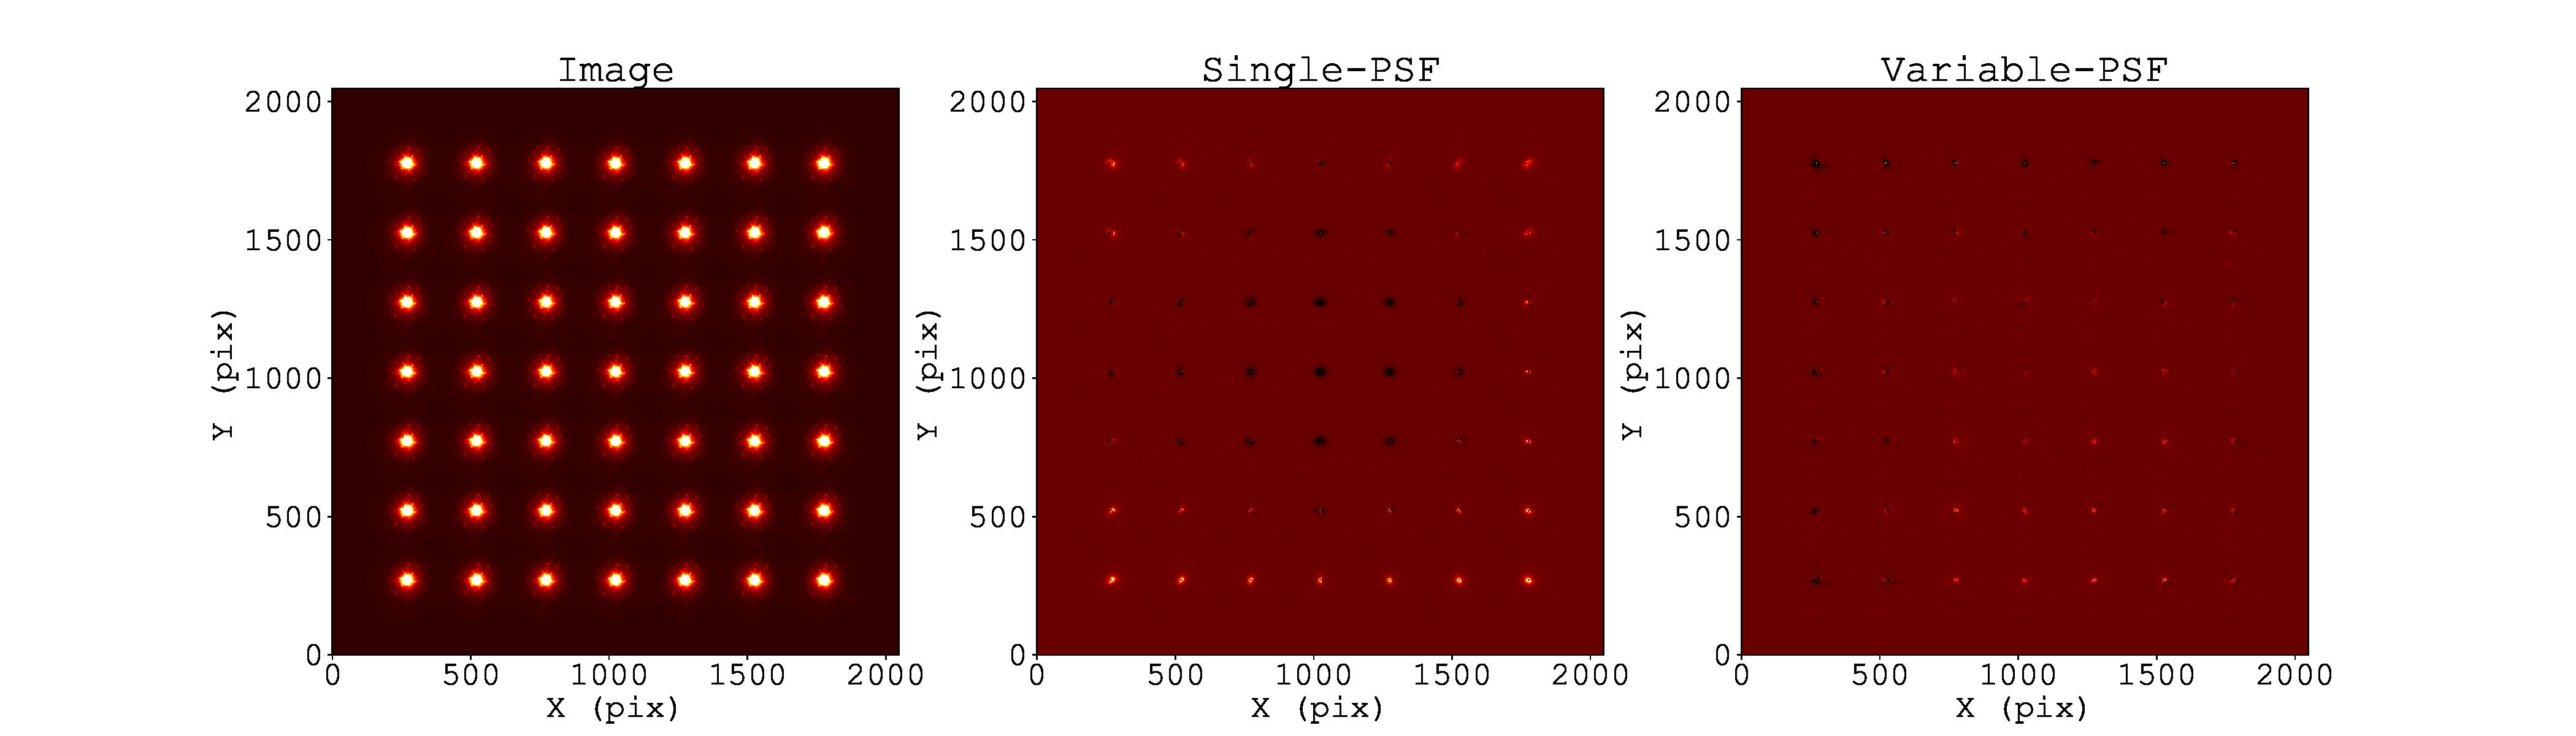
\includegraphics[width=1.3\textwidth]{airopa/Figures/osiris_star_grid.pdf}
 }
 \caption{\footnotesize Simulated grid of stars on the OSIRIS imager (\textit{left}), residual image from the single-PSF mode (\textit{middle}) and variable-PSF mode (\textit{right}). \label{fig:grid_stars}}
\end{figure}

\begin{figure}[!h]
  \subfloat{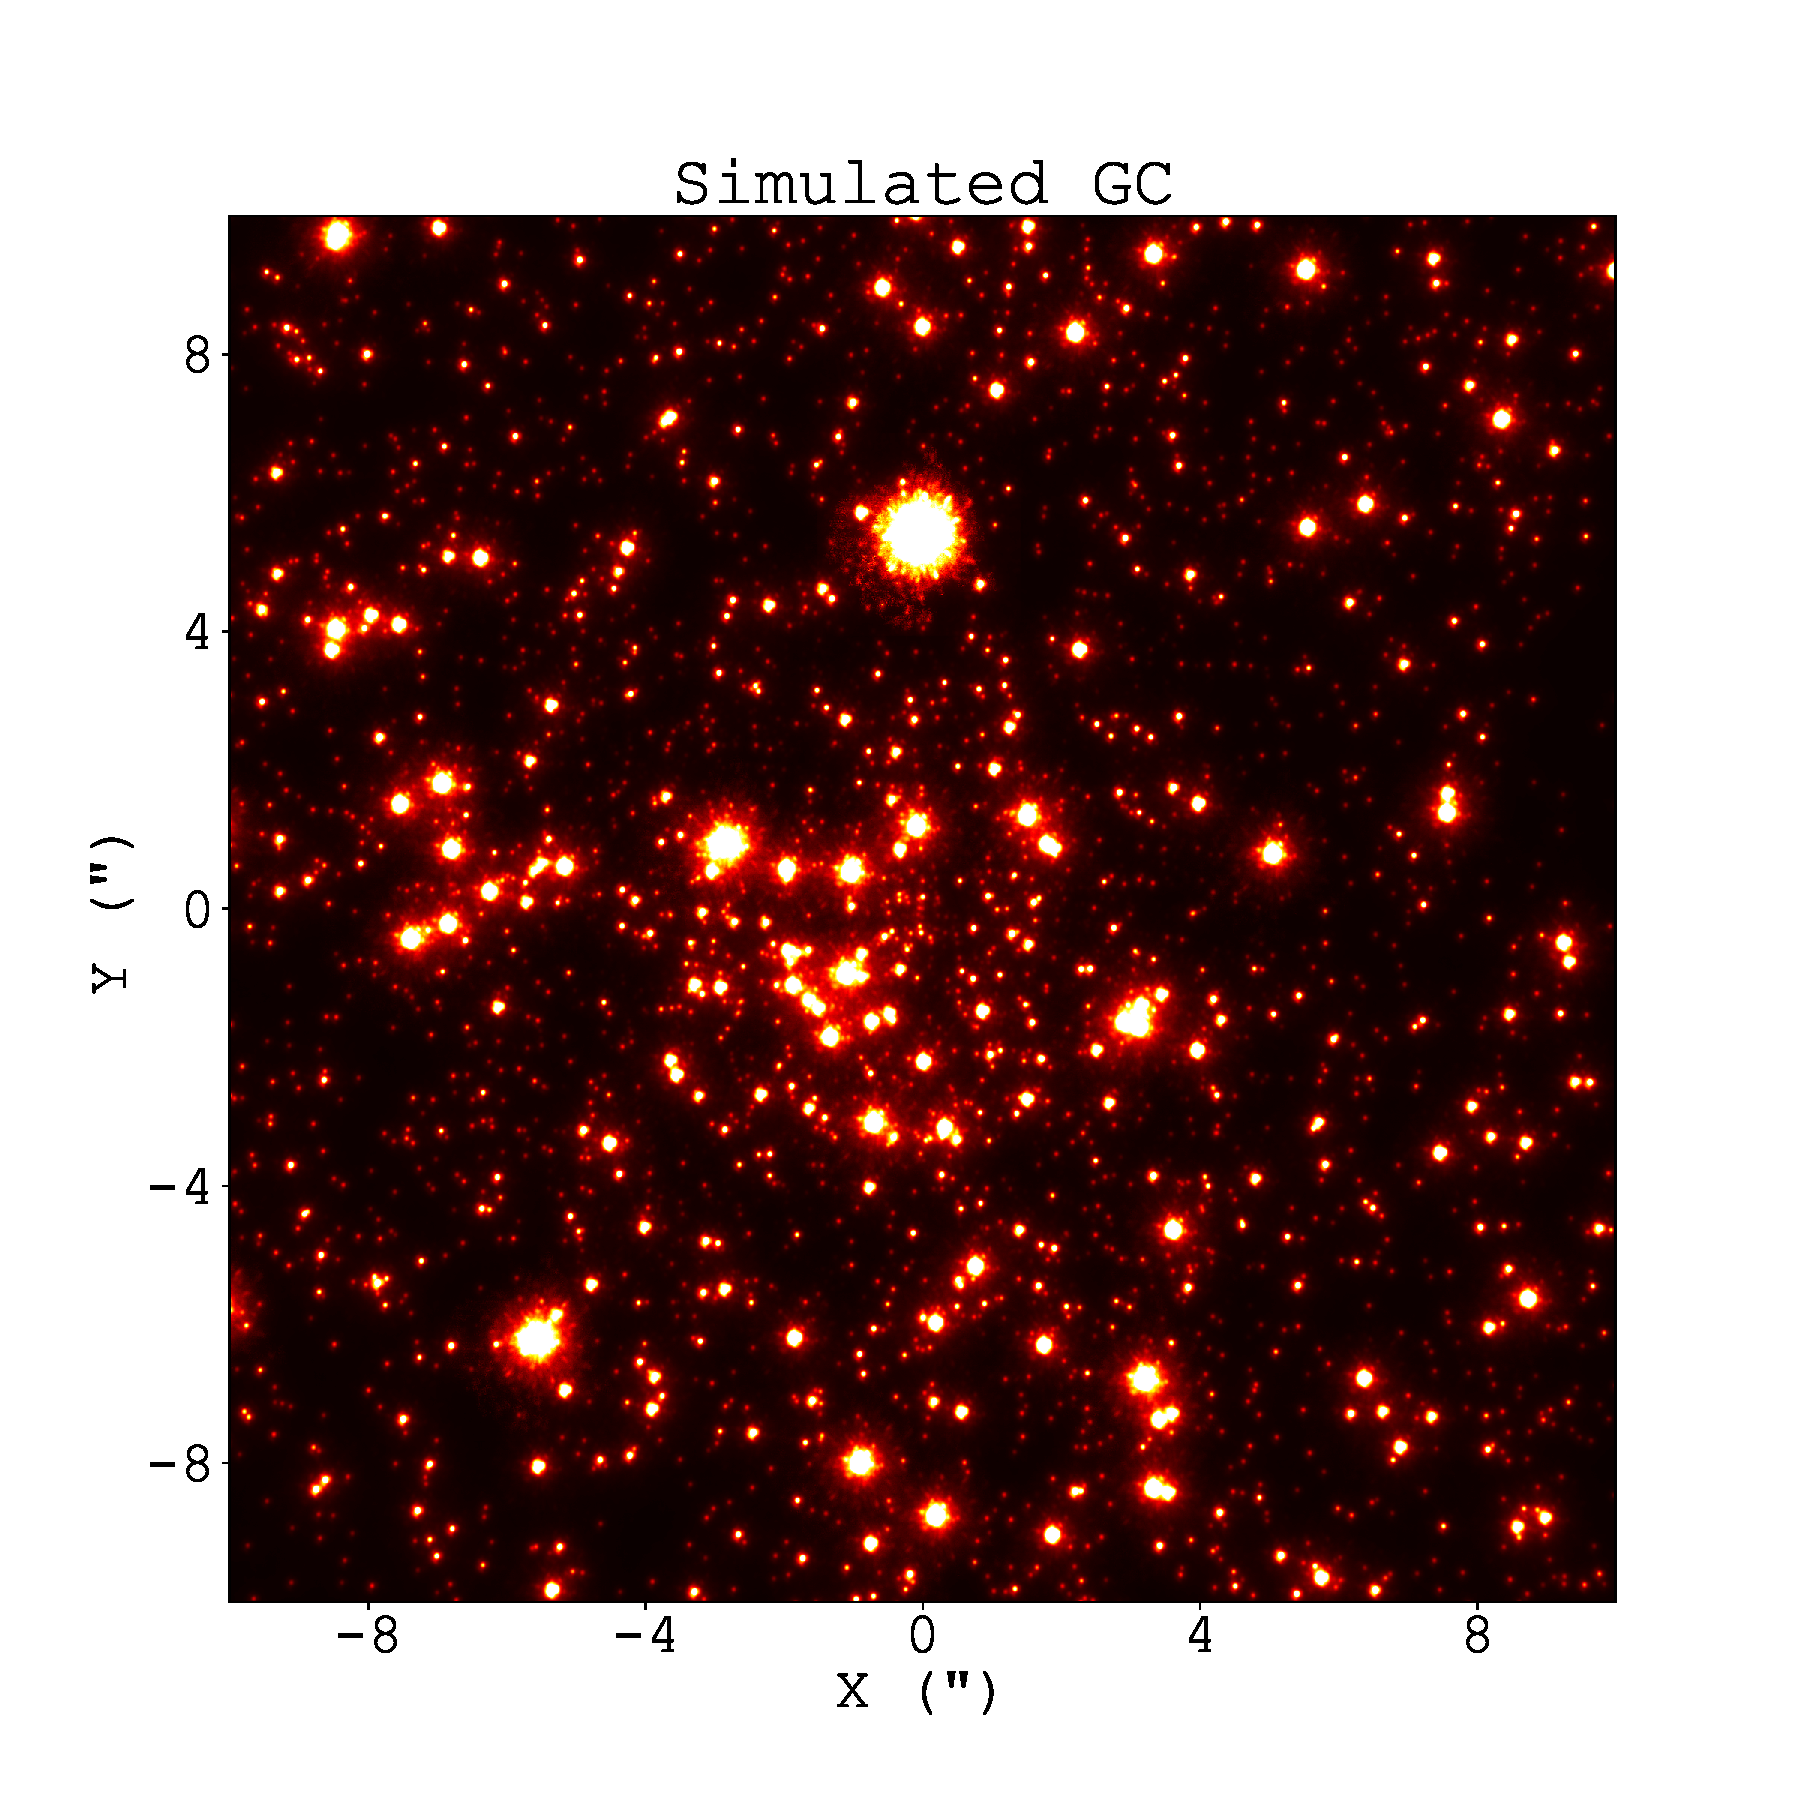
\includegraphics[width=0.9\textwidth]{airopa/Figures/synthetic_gc_osiris.pdf}}
  \caption{\footnotesize \textit{Left}: On-sky OSIRIS image of the GC, with a dashed yellow outline representing the NIRC2 field of view. \textit{Right}: Full-frame NIRC2 image of the central ${\sim}10$ arcseconds around the GC.} \label{fig:gc_osiris_nirc2}
\end{figure}

\section{On-sky Observations}\label{sec:on_sky_obs}
The datasets presented in this work were acquired with the Keck-II/OSIRIS imager in the laser guide star adaptive optics (LGSAO) mode. The data were taken with the K$_{\textrm{p}}$ filter ($\lambda_{c} = 2.12\mu$m), the pixel scale for the OSIRIS imager is 9.952 mas/pix, and all of the data (including phase diversity) were taken in 2020. Figure BBB shows an individual cleaned frame from our galactic center (GC) observations with OSIRIS.

\begin{figure}[!h]
  \hspace{-20mm}
  \subfloat{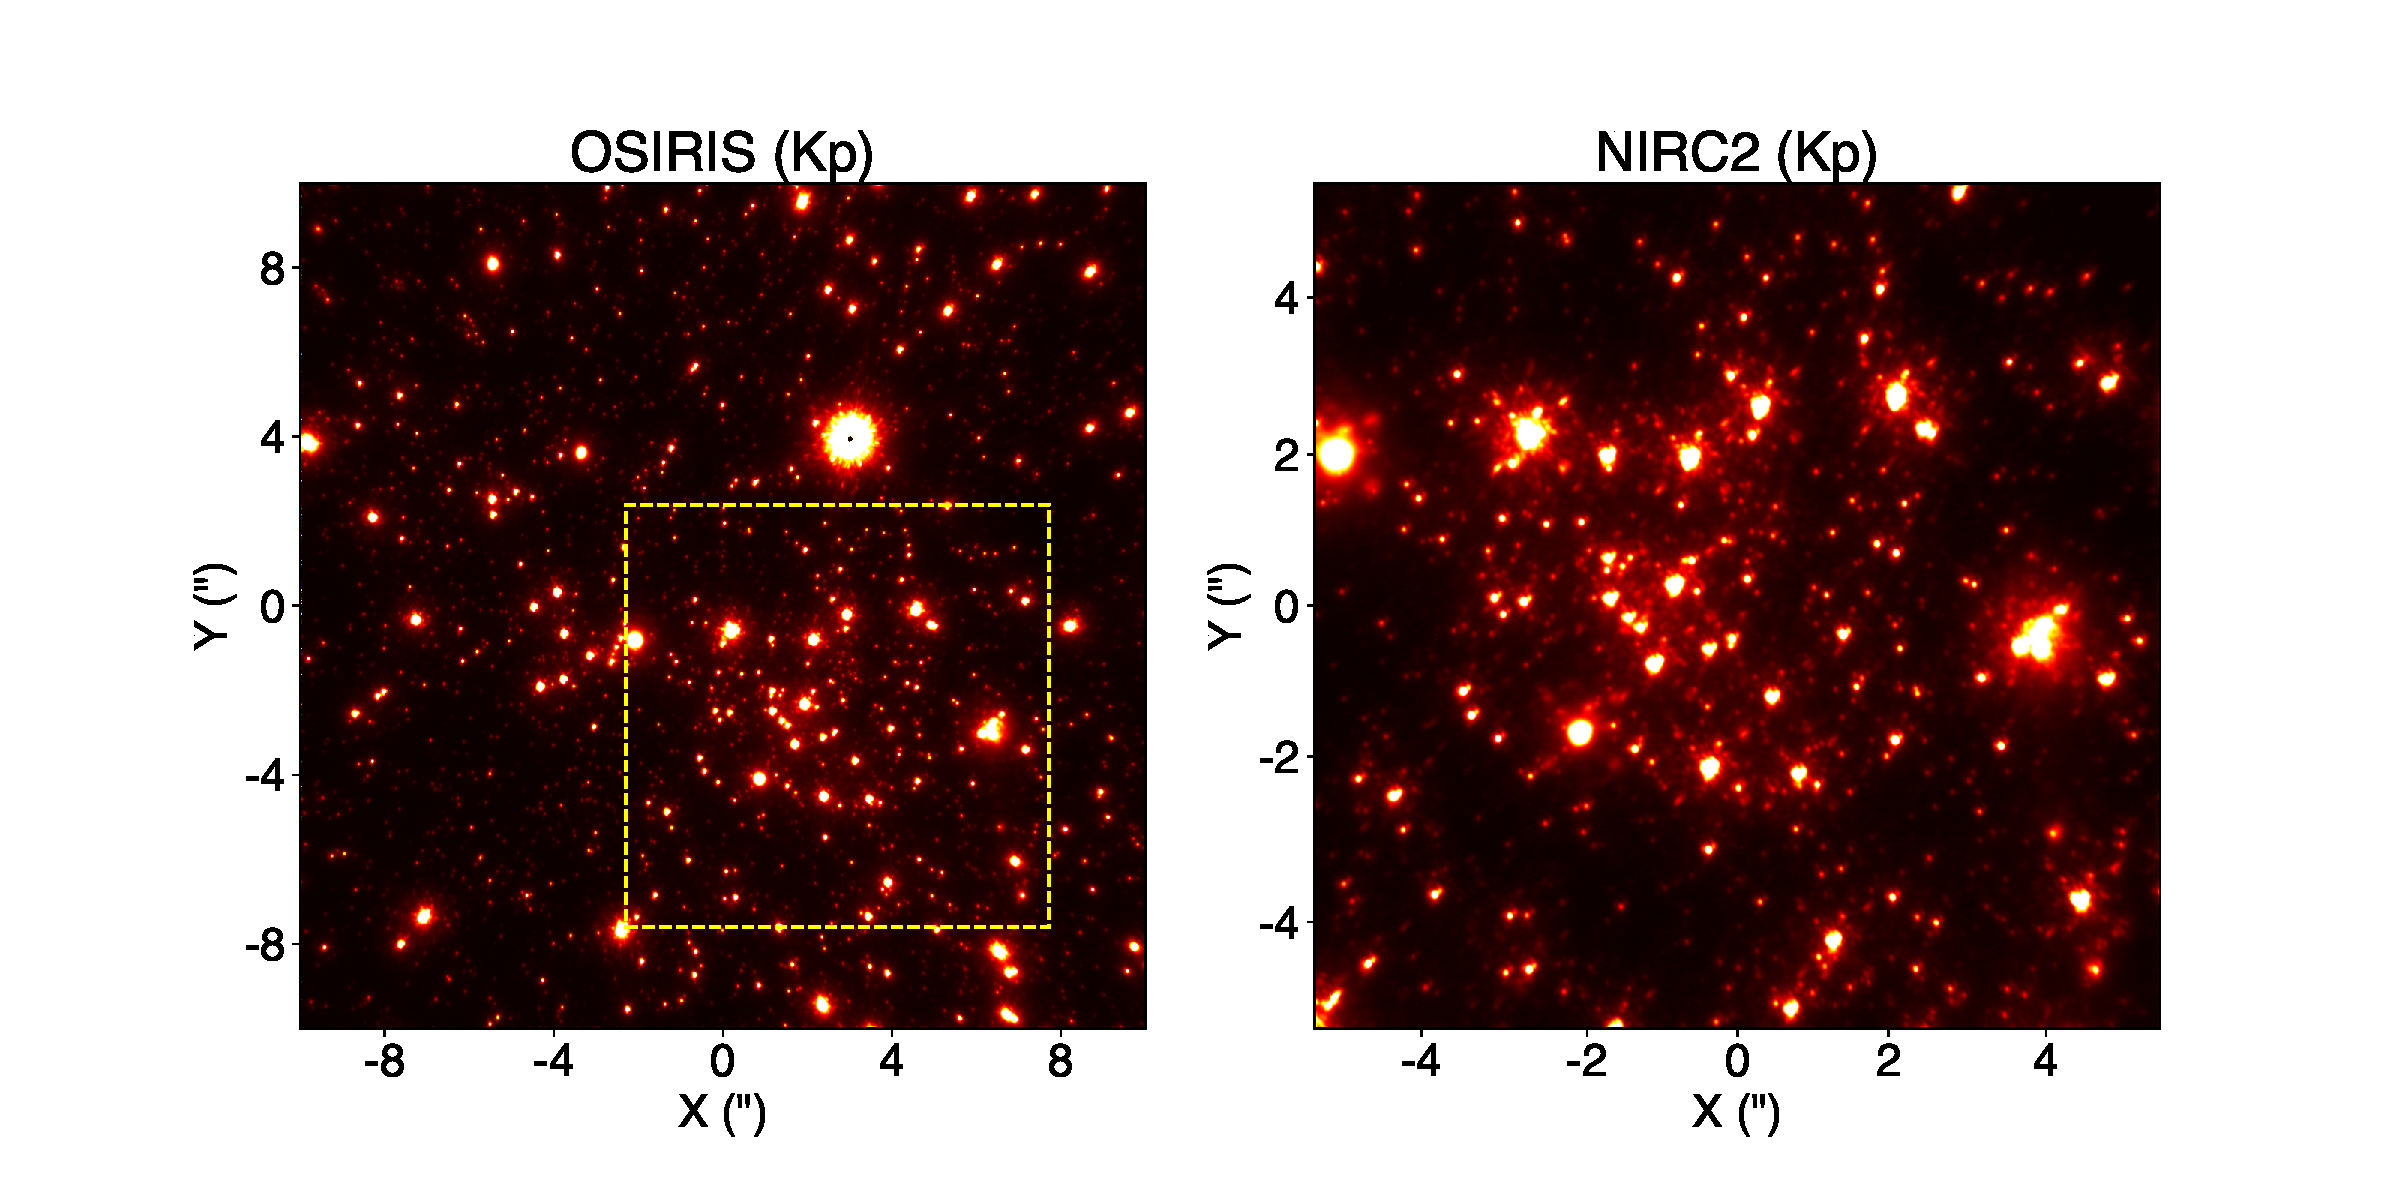
\includegraphics[width=1.2\textwidth]{airopa/Figures/gc_osiris_nirc2_image.pdf}}
  \caption{\footnotesize \textit{Left}: On-sky OSIRIS image of the GC, with a dashed yellow outline representing the NIRC2 field of view. \textit{Right}: Full-frame NIRC2 image of the central ${\sim}10$ arcseconds around the GC.} \label{fig:gc_osiris_nirc2}
\end{figure}

\section{Results}\label{sec:results}
Present the overall results for AIROPA on OSIRIS GC data. Compare astrometric/photometric precision, FVU, etc.

\section{Discussion and Conclusion}\label{sec:conclusion}
Present the overall results for AIROPA on OSIRIS GC data. Compare astrometric/photometric precision, FVU, etc.

% References
\bibliography{refs} % bibliography data in report.bib
\bibliographystyle{spiebib} % makes bibtex use spiebib.bst

\listoffigures

\end{document} 
